% !TeX spellcheck = en_US
\documentclass[sigconf,nonacm]{acmart}
\usepackage{listings}
\settopmatter{printacmref=false}
\pagestyle{empty}
\AtBeginDocument{%
  \providecommand\BibTeX{{%
    \normalfont B\kern-0.5em{\scshape i\kern-0.25em b}\kern-0.8em\TeX}}}
\copyrightyear{2020}
\acmYear{2020}
\setcopyright{rightsretained}
\begin{document}
\title{Deep Learning for Visual Computing}
\subtitle{Exercise 1: Linear Model}
\author{SHU Yuting}
\email{e11931687@student.tuwien.ac.at}
\affiliation{Mat.Nr. 11931687}
\author{Helmuth BREITENFELLNER}
\email{helmuth.breitenfellner@student.tuwien.ac.at}
\affiliation{Mat.Nr. 08725866}
\begin{abstract}
In this assignment we have been creating a linear classifier for images
distinguishing between cats and dogs.
The linear classifier was then trained, using random search for good
parameters of learning rate and momentum, and evaluated against the
validation set.
The best model was then evaluated against the test set.
\end{abstract}
\keywords{Deep Learning, Linear Model, Visual Computing, Image Processing, PyTorch}
\maketitle
\section{Task description}
Based on a skeleton we were tasked to implement a simple classification
of images between \emph{cats} and \emph{dogs}.
For this, the CIFAR10\footnote{\url{https://www.cs.toronto.edu/~kriz/cifar.html}}
has been downloaded and split into a training, testing and validation
set.

The training was implemented using batched gradient descent with
momentum, based on Nesterov's accelerated gradient descent
(Nesterov, 1983 \cite{Nes83}).

For the creation of batches we chose a size of 512 images.
This seems to be a good compromise between speed of training,
while bringing the benefit of stochastic gradient descent
(added noise at training to avoid local minima).

We experimented with performing the training on a GPU,
however due to the simplicity of the model the execution times using
GPU were actually larger.
Therefore we have performed all calculations on CPU.

\section{Image Classification}

Image classification is the process to identify and categorize images
into classes.

According to the target class, we could divide image classification into three categories, binary image classification, multi-class image classification and multi-label image classification.

Binary image classification separates images into exactly one of two classes. And in multi-class image classification, an image is assumed to belong to exactly one of more than two classes, and
in the process of the image classification the class of an image
is identified.

In multi-label classification, there are two classes or more and every image belongs to one or multiple classes at the same time. For instance, guess the genre(action, drama, comedy, etc.) of a movie from a wall poster.

The individual image is often called "sample", and the corresponding
class is called "label".
If the label is predicted by the image classification process
and not necessarily corresponds to the real class it is
called "prediction".

\section{Purpose of Training, Testing and Validation Sets}

When performing machine learning, it is useful to have a training,
validation and test data set.

The \emph{training set} is used to learn the model. By using this model
the learning algorithm (e.g. gradient descent) optimizes the parameters
(e.g. weights) to minimize the error.

Would the model be evaluated against the training set, it would be
incentivized for memorizing the samples and their corresponding labels.
However, the goal is to get good performance for predicting
the labels of unknown samples, therefore a set of samples which is
disjoint from the training set, called \emph{validation set}, is used to
evaluate the quality (e.g. accuracy, precision, recall, F1, ...)
of the model.

The \emph{validation set} is used to tune the process. For example it can used
to perform early stopping in the learning, as well as for finding good
values of \emph{hyperparameters} (these are parameterizations of the process
which are not optimized during the learning phase).

Since the validation set is used for tuning the hyperparameters, it
indirectly influences the model.
To get a real estimate of the performance of the model when used to
predict labels of \emph{unseen} samples one uses a third set, the
\emph{test set}.
This third set is disjoint to both the training and the validation set.
This means that every sample is in only one of the three sets
training, test, or validation.
The test set is ideally used only \emph{once}, after the learning
of the parameters
and the optimization of the hyperparameters, to evaluate the performance
of the model.

\emph{Alternatively one can use cross-validation together with a test data set.
However, in the area of deep learning the training times for models are so
large that cross-validation is not practicable.}

\section{How Linear Classifiers Work}

Linear classifiers use a linear combination of the feature values
to predict a score for each of the classes.
Afterwards one can choose the class with the highest score
as the "prediction", or one can calculate out of the scores
"probabilities", by applying a soft-max on the final set of scores.

The parameters of a linear classifier are the weights of the linear
combinations.
Usually one also adds a constant to each score, the so-called \emph{bias}
vector.

To get the weights of the linear classifier, they are iteratively
adjusted to minimize the loss, i.e. the error of the classification
on a sample or a batch of samples.
One approach is gradient descent, where the weights are modified
in the opposite direction of the gradient of the loss as a function
of the weights.

Linear classifiers can also be interpreted geometrically.
In the most simple case of two classes a linear classifier defines
a hyperplane in the hyperspace of the features.
On one side of the hyperplane is the class $A$,
on the other side is the class $B$.

For more classes one can imagine a set of hyperplanes, one per class.
The hyperplane for class $X$ cuts the hyperspace into an area
where the probability of \emph{is in class $X$} is high,
and another area where the probability of \emph{is in class $X$}
is low.
The distance from the hyperplane is then corresponding to the
probability of \emph{being in $X$} or \emph{not being in $X$},
depending on which side of the hyperplane the sample lies.

\section{Results from \texttt{linear\_cats\_dogs.py}}
We have been performing a random search for good hyperparameter
values of the learning rate and the momentum, by trying 100 random
values (logarithmic scale for learning rate, linear scale for momentum).

These were the results obtained from training and evaluating
the simple linear model:
\begin{lstlisting}[basicstyle=\ttfamily\small]
Validation: accuracy: 0.6031357177853993
Parameters: momentum=0.869774239381628
            lr=0.3726148634713726
Test: accuracy: 0.6135
\end{lstlisting}

The following plot tries to depict the influence of the hyperparameters
on the validation
accuracy.

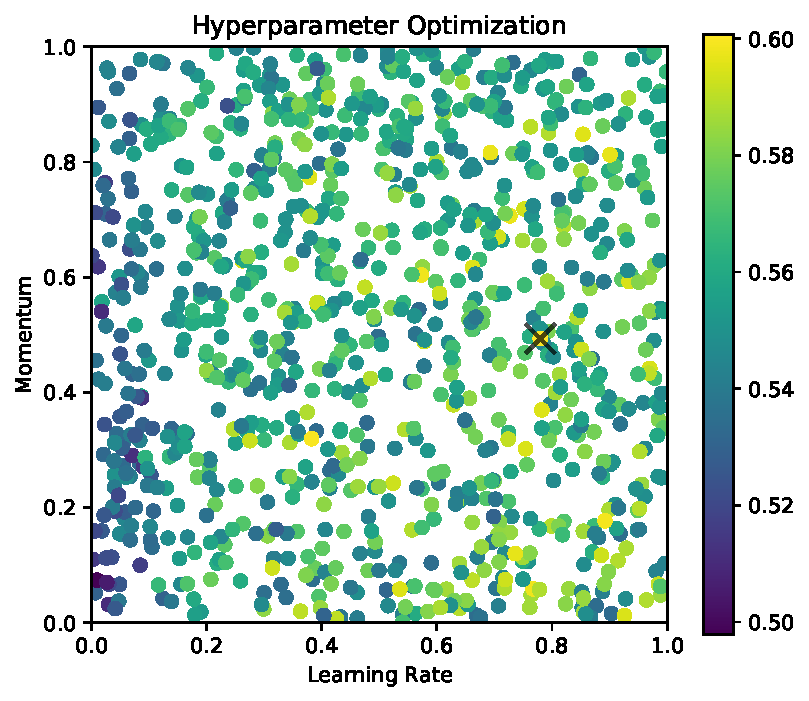
\includegraphics[width=0.5\textwidth]{plot.pdf}

\bibliographystyle{ACM-Reference-Format}
\bibliography{report}
\end{document}
